% !TeX spellcheck = en_US
\chapter{Introduction}

\todo{maybe prologue?}

\section{Motivation}

\todo{Motivation}

\section{The IceCube Neutrino Observatory}

Since January 2011, the IceCube Neutrino Observatory at the South Pole is measuring neutrinos emanating from various sources. For this purpose a detector instrumented with digital optical modules (\enquote{DOMs}) is installed deep in the antarctic ice. 5160 of these optical sensors are arranged on 86 strings at a height between \SI{1450}{\meter} and \SI{2450}{\meter} below the surface. The central region of this In-Ice Array which has a higher density of DOMs is called \enquote{DeepCore}. Figure \ref{icecube:detector} shows a sketch of the detector arrangement.

\begin{figure}[h]
	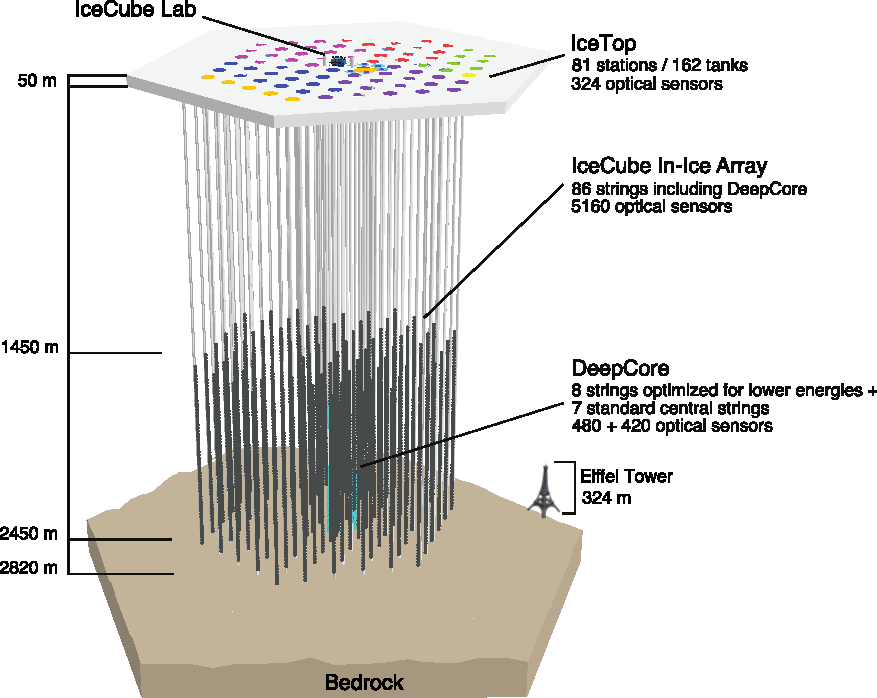
\includegraphics[width=\textwidth]{IceCubeDetector.pdf}
	\caption[Schematic view of IceCube]{\textbf{Schematic view of the IceCube Neutrino Observatory. \cite{icecube:instrumentation}} The in-ice array with the denser sub-array DeepCore as well as the surface array IceTop is sketched. Different station colors represent different deployment stages.}
	\label{icecube:detector}
\end{figure}

Neutrinos are very interesting elementary particles because of their weak interaction cross section and their electrical neutrality. This fact makes it possible for neutrinos to let them point back to their sources which is exploited in the search for astrophysical processes like active galactic nuclei, supernovae, or gamma-ray bursts. Since they are able to reach us without scattering processes, neutrinos can even give information about sources at cosmological distances. Simultaneously, the weak interaction potential is what neutrino detection makes challenging. Therefore, a detector with a large scale active volume is needed. In the case of IceCube, this is \SI{1}{\cubic\kilo\meter} of ice.

At the surface on top of the in-ice detector the cosmic ray air shower array IceTop is installed to detect Cherenkov radiation (see \ref{sec:cherenkov}). IceTop consists of 81 stations approximately arranged in the same grid as the in-ice strings. Each station has two tanks filled up with ice and two standard IceCube DOMs. This arrangement makes it possible for IceTop to detect primary cosmic rays (see \ref{sec:cosmicrays}) in the energy range of \si{\peta\electronvolt} to \si{\exa\electronvolt}. One purpose of IceTop is to provide a veto for downward-going neutrinos in the IceCube detector originating from coincident atmospheric air shower events. \cite{icecube:instrumentation} Since IceCube is investigating astrophysical neutrinos, atmospheric neutrinos are a major background.

\section{Cosmic Rays}\label{sec:cosmicrays}

Charged particles or nuclei that are propagating through the universe and incidentally reach the Earth's atmosphere are called cosmic rays. They were discovered by the Austrian physicist \textsc{Victor Franz Hess} in 1912 when he observed an increasing discharge of electroscopes with increasing height in seven ballon flights. \cite{cosmicrays:hess} Hess initially called this underlying radiation \enquote{durchdringende Strahlung} (\textit{penetrating radiation}).

\begin{figure}[h]
	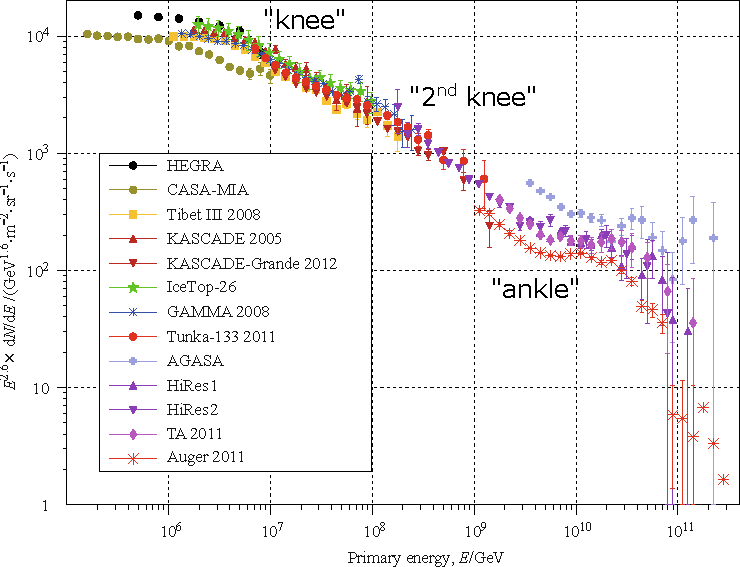
\includegraphics[width=\textwidth]{CosmicRayEnergySpectrum.pdf}
	\caption[Cosmic ray energy spectrum]{\textbf{Energy spectrum of cosmic rays measured with multiple air shower experiments. \cite[adapted]{cosmicrays:gaisser}} The three prominent regions known as \enquote{knee}, \enquote{second knee}, and \enquote{ankle} are marked. Multiplication of the spectrum by the factor $E^{2.6}$ leads to a better visibility and shows that the spectral index changes at these features.}
	\label{cosmicrays:spectrum}	
\end{figure}

When it comes to cosmic rays, ascertaining the mass composition is a key measurement for learning about their propagation in universe and about extra-galactic cosmic ray accelerators. Figure~\ref{cosmicrays:spectrum} shows that the energy spectrum of cosmic rays follows a power law:
\begin{align}
\frac{dE}{dN}\propto E^\gamma\,,
\end{align}
introducing a spectral index $\gamma$ which is dependent from the considered energy region.
Due to this interesting features, composition measurements at these \enquote{transition points} are desired in particular.

Due to the shape the spectrum is referred to as \textit{poly gonato} (Greek for \enquote{many knees}). The \enquote{knee} is assumed to be based on different rigidity\footnote{property of a magnetic field to bend a particle's trajectory} dependent cut-off energies for sub-spectra of element groups which sum up to the spectrum we observe. \cite{cosmicrays:hoerandel, cosmicrays:shapiro} At energies beyond \SI{e11}{\giga\electronvolt} a strong suppression is observed. The GZK-effect (named after Kenneth \textsc{Greisen}, Georgiy \textsc{Zatsepin}, and Vadim \textsc{Kuzmin}) is supposed to be the reason. Protons with energies above a threshold of \SI{5e19}{\electronvolt} can interact with photons of the cosmic microwave background in such a way that they produce $\pi^0$ and $\pi^+$ mesons via $\Delta^+$ resonance:
\begin{align}
\gamma_\text{CMB} + p \rightarrow \Delta^+ &\rightarrow p + \pi^0\\
&\rightarrow n + \pi^+\,.
\end{align}
Thus, the protons effectively lose about \SI{20}{\percent} of their energy. Additionally, calculations show that these interactions become quite frequent for proton energies of $E_p\gtrsim\SI{e20}{\electronvolt}$ which results in an effective cutoff of cosmic-ray energies above this region. \cite{cosmicrays:gzk}

\section{Extensive Air Showers}

If a high energetic particle -- a photon or hadron -- incidentally reaches the Earth's atmosphere, it interacts with their atoms. A common way to describe the traversed atmospheric matter for an air shower is the \textit{slant depth}

\begin{align}
X(h) = \int_{h}^{\infty}\rho(h')dh'
\end{align}
 
\begin{figure}[h]
	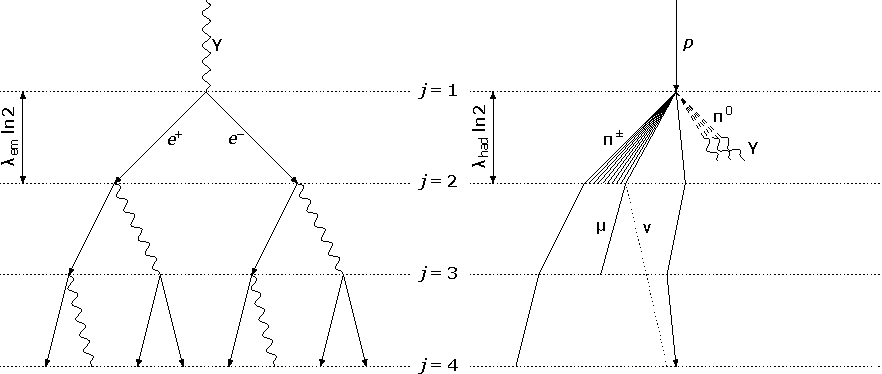
\includegraphics[width=\textwidth]{AirShowerHeitler.pdf}
	\caption[Schematic view of extensive air showers]{\textbf{Schematic view of extensive air showers. \cite{famous:niggemann}}}	
\end{figure}

\section{Detection of Air Showers via Atmospheric Cherenkov Light}\label{sec:cherenkov}

\subsection{The Cherenkov Effect}

\begin{figure}[h]
	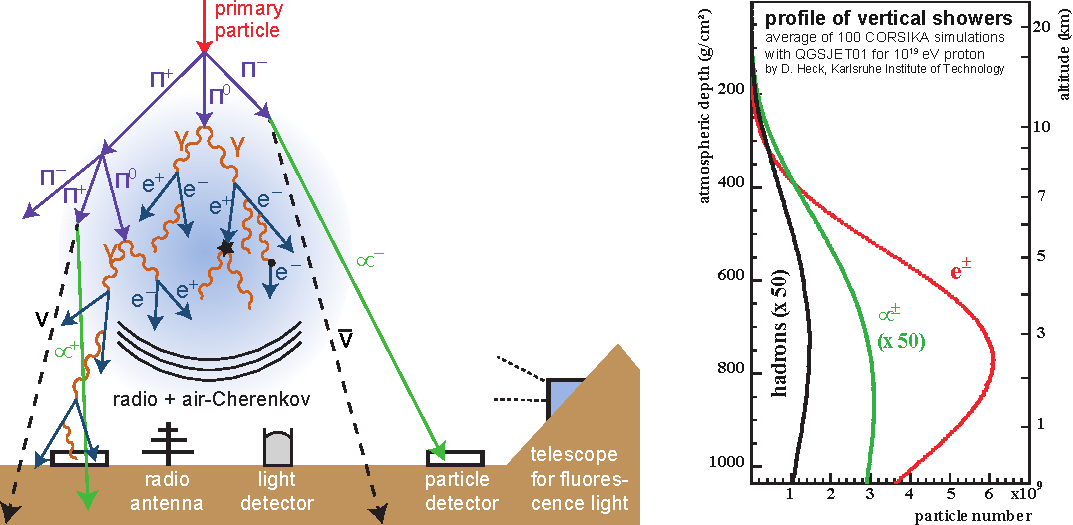
\includegraphics[width=\textwidth]{AirShowerDetection.pdf}
	\caption[Different techniques for air shower detection]{\textbf{Different techniques for the detection of atmospheric air showers. \cite{airshowers:schroeder}} }	
\end{figure}

\section{Imaging Air Cherenkov Telescopes}

\subsection{Imaging Technique}

\subsection{Photon Detection}

\subsection{IceAct}